\NeedsTeXFormat{LaTeX2e}
\documentclass[a4paper,12pt,
headsepline,           % Linie zw. Kopfzeile und Text
oneside,               % einseitig
pointlessnumbers,      % keine Punkte nach den letzten Ziffern in Überschriften
bibtotoc,              % LV im IV
%DIV=15,               % Satzspiegel auf 15er Raster, schmalere Ränder   
BCOR15mm               % Bindekorrektur
]{scrbook}
\KOMAoptions{DIV=last} % Neuberechnung Satzspiegel nach Laden von Paket helvet

\pagestyle{headings}
\usepackage{blindtext}

% für Texte in deutscher Sprache
\usepackage[english]{babel}
\usepackage[utf8]{inputenc}
\usepackage[T1]{fontenc}

% Helvetica als Standard-Dokumentschrift
\usepackage[scaled]{helvet}
\renewcommand{\familydefault}{\sfdefault} 

% Literaturverzeichnis mit BibLKaTeX
\usepackage[babel]{csquotes}
\usepackage[backend=bibtex8,sorting=none,style=numeric-comp]{biblatex}
\bibliography{bibliography-prj}
\renewcommand*{\bibfont}{\small}

\usepackage{tikz}
\tikzset{every picture/.style={line width=0.75pt}} 

\usepackage{graphicx}
\usepackage{tabularx}
\usepackage{booktabs}
\usepackage{siunitx}
\usepackage{longtable}
\usepackage{multirow}
\usepackage{multicol}
\usepackage{float}
\usepackage{subfig}
\usepackage{dblfloatfix}

% Besondere Schriftauszeichnungen
\usepackage{xurl}              % \url{http://...} in Schreibmaschinenschrift
\usepackage{color}            % zum Setzen farbigen Textes
\usepackage{xcolor}
\usepackage{nicefrac}
\usepackage{amssymb, amsmath, amsthm} % Pakete für Mathe-Umgebungen und -Symbole

\newtheorem{definition}{Definition}

\usepackage{setspace}         % Paket für div. Abstände, z.B. ZA
\setlength{\parindent}{0pt}   % kein linker Einzug der ersten Absatzzeile
\setlength{\parskip}{1.4ex plus 0.35ex minus 0.3ex} % Absatzabstand, leicht variabel

% Tiefe, bis zu der Überschriften in das Inhaltsverzeichnis kommen
\setcounter{tocdepth}{3}      % ist Standard

% Beispiele für Quellcode
\usepackage{listings}
\definecolor{codegreen}{rgb}{0,0.6,0}
\definecolor{codegray}{rgb}{0.5,0.5,0.5}
\definecolor{codepurple}{rgb}{0.58,0,0.82}
\definecolor{backcolour}{rgb}{0.95,0.95,0.92}
\lstset{
	backgroundcolor=\color{backcolour},   
	commentstyle=\color{codegreen},
	keywordstyle=\color{magenta},
	numberstyle=\tiny\color{codegray},
	stringstyle=\color{codepurple},
	basicstyle=\ttfamily\footnotesize,
	breakatwhitespace=false,         
	breaklines=true,                 
	captionpos=b,                    
	keepspaces=true,                 
	numbers=left,                    
	numbersep=5pt,                  
	showspaces=false,                
	showstringspaces=false,
	showtabs=false,                  
	tabsize=2
}
\renewcommand{\lstlistingname}{Source Code}

\usepackage{booktabs}

% hier Namen etc. einsetzen
\newcommand{\fullname}{Jonathan Schilling}
\newcommand{\email}{jonathan.schilling@uni-ulm.de}
\newcommand{\titel}{Analysis of gameplay from the video game Valorant} 
\newcommand{\jahr}{2023}
\newcommand{\matnr}{980556}
\newcommand{\gutachterA}{Prof.\,Dr.\,Friedhelm Schwenker}
\newcommand{\betreuerB}{}
\newcommand{\betreuerA}{}
% hier die Fakultät auswählen
\newcommand{\fakultaet}{Engineering, Computer Science und Psychology}
% hier das Institut einsetzen
\newcommand{\institut}{Institute of Neural Information Processing}

% Informationen, die LaTeX in die PDF-Datei schreibt
\pdfinfo{
  /Author (\fullname)
  /Title (\titel)
  /Producer     (pdfeTex 3.14159-1.30.6-2.2)
  /Keywords ()
}

\definecolor{dark blue}{HTML}{000066}

\definecolor{todoCite}{HTML}{ABD4B6}%Quellen raussuchen
\definecolor{todoRef}{HTML}{A7C5DB}%Auf glossar, acronyme, bilder etc referenzieren
\definecolor{todoNorm}{HTML}{E6C59E}%Sonstige Todos
\definecolor{todoCont}{HTML}{B483C9}%Inhalte

\usepackage[hyperfootnotes=false]{hyperref}
\usepackage[multiple]{footmisc}
\usepackage[all]{hypcap}
\hypersetup{
pdftitle=\titel,
pdfauthor=\fullname,
pdfsubject={Project Thesis},
pdfproducer={pdfeTex 3.14159-1.30.6-2.2},
colorlinks=false,
linkcolor=dark blue,
citecolor=dark blue,
pdfborder=0 0 0	% keine Box um die Links!
}

\usepackage[toc,nonumberlist,nopostdot,nomain,acronym]{glossaries}\makeglossaries
%\newacronym[longplural={}]{acr-label}{short}{long}

\newacronym[description=Application Programming Interface]{acr-api}{API}{application 
programming interface}
\newacronym[name=mAP]{acr-mAP}{$mAP$}{Mean Average Precision}
\newacronym{acr-iou}{IoU}{Intersection over Union}


% Trennungsregeln
\hyphenation{Hy-phe-na-tion}

\begin{document}
\frontmatter

% Titelseite
\thispagestyle{empty}
\begin{addmargin*}[4mm]{-1mm}
	
	
\includegraphics[height=1.8cm]{images/unilogo_bild}
	\hfill
	
\includegraphics[height=1.8cm]{images/unilogo_wort}\\[1em]
	
	{\footnotesize
		%{\bfseries Universität Ulm} \textbar ~89069 Ulm \textbar ~Germany
		\hspace*{99mm}\parbox[t]{44mm}{\bfseries Faculty of \fakultaet\\
			\mdseries \institut}\\[2cm]
		
		\parbox{143mm}{\bfseries \LARGE \titel}\\[2.5em]
		{\footnotesize Project Report at Ulm University}\\[3em]
		
		{\footnotesize \bfseries Submitted by:}\\
		{\footnotesize \fullname\\ \email}\\ \matnr\\[2em]
		{\footnotesize \bfseries Examiner:}\\                     
		{\footnotesize \gutachterA}\\[2em]
%		{\footnotesize \bfseries Betreuer:}\\ 
%		{\footnotesize \betreuerA\\ \betreuerB}\\\\
		{\footnotesize \jahr}
	}
\end{addmargin*}


% Impressum
\clearpage
\thispagestyle{empty}
{ \small
	\flushleft
	Edition: \today \\\vfill
	\copyright~\jahr~\fullname
}
% ab hier Zeilenabstand etwas größer 
\setstretch{1.2}

\tableofcontents

\mainmatter
\chapter{Introduction}\label{chpt:introduction}
\glsresetall

E-Sports is a growing market for years. The events become more professional, prize money is rising 
and even broadcasters like ProSieben MAXX already show such events on 
television~\cite{kovacevic}. In light of this, the performance pressure of teams get bigger and 
preparation effort increases. But what exactly is e-sports? The German Games Industry Association 
defines the term e-sports as a competition between two or more people playing video games 
according to fixed rules~\cite{kovacevic}. Those people are mostly organized in professional teams 
from all around the world. Common game genre for e-sports events are real-time strategy games, 
multiplayer online battle arena games, tactical shooters and sport simulations. For popular games 
like League of Legends (Riot Games), Counter Strike: Global Offensive (Valve) or FIFA (Electronic 
Arts)  various leagues and tournaments were founded and the players have to show their best 
performances to keep their place in the team as professional gamer. During the corona pandemic 
online content streaming on platforms like Twitch or Mixer became very popular and also the 
popularity of e-sports was boosted, which often is streamed on such platforms~\cite{kovacevic}. In 
that time a new tactic shooter was published: Valorant from Riot Games~\cite{riotgames-valorant}. It 
became a big hype and therefore the player base grew very fast, so that Riot Games decided to start 
a tournament the "Valorant Champions Tour" also called VCT~\cite{riotgames-vct}. A concept and 
first implementation for a tool that can help Valorant teams and players to improve their performance 
in e.g. the highly competitive VCT is introduced in this project report.

\section{Problem Definition}\label{sec:intro:problem}

After that short introduction to e-sports in general, the following section defines the problem that is 
addressed within that project. The initial idea of that project came from a Youtube 
video~\cite{river2021} in that someone tried to implement an artificial intelligent agent that plays the 
video game Valorant autonomously.
Such agents in general are a big problem in the gaming scene because some players try to gain an 
unfair advantage from 3rd party programs. Those programs are used to display more information for 
the players than intended or helps them to react faster and more precise on occurring events than it 
is possible for a human being. Due to that problem it is prohibited in the terms and conditions of 
online multiplayer games to use any type of additional programs to play the game. Furthermore there 
are anti-cheat mechanisms running on the same computer as the game, searching for suspect 
programs that try to manipulate the outcome of a match. If a cheat program is detected the player 
becomes banned from the game. Because of that fact it is not that easy to implement and test an 
artificial agent that plays the game.

Due to cheating concerns the video and its content could be condemned but the creator just had 
educational purposes, did not harmed any player and in the end the implemented agent would not be 
good enough to compete with average Valorant players. In the video the creator found a way that he 
could implement an agent that cannot be detected by the anti-cheat mechanisms: he placed the 
agent on a separate computer than the game. Additionally in difference to programs that try to 
cheat, the artificial agent only became the ability to interact with the game client as every human 
player. Input was the content of the in-game screen, captured completely legal and output of the 
agent were mouse and keyboard commands, that were transmitted to the computer with the 
Valorant client running. With that setup he successfully created a system that was able to play the 
game on a very basic level. Due to the reason that he showed a way that could make it possible to 
build a cheat-client that cannot be detected by the anti-cheat of Valorant he decided not to share 
his source code~\cite{river2021}.

So the first idea of the project was to recreate a similar agent, but that would have been too much 
for a single project. Therefore the next idea was to build an application that is able to 
analyze Valorant gameplay and helps to evaluate already played games for training purposes, as it is 
common in most ordinary sport disciplines. The task of that application is to generate alternative 
representations of game data. Normally data from matches is available as recorded video from 
player respectively observer view or as raw data saved in databases from the game publisher. A 
transformation of those data can result in a better overview and understanding of the whole match 
and what happens there. In a first step those generated transformations can be analyzed by a trainer 
or the players themselves. Later it would be possible to use this data again as input for other pattern 
recognition algorithms that try to find problems in rounds that were lost and flaws in the tactics of 
opponents or even to invent new tactics. Further it could be possible to train an artificial agent with 
such transformations as input and try to reach a new level of tactical understanding.

As already mentioned one possibility to get game data are databases from the game publisher. 
There is also an \gls{acr-api} that would provide all data from matches but it is impossible to get an 
\gls{acr-api}-Key if it is not used for an already publicly running and from Riot Games legitimated 
application. For this reason the raw data will be gameplay videos that become transformed into a 
simpler form of presentation.

Summarized the task of that project is to use a pattern recognition algorithm to transform a 
gameplay video of the computer game Valorant into a more compact and easier to understand data 
representation. That includes acquisition and pre-processing of data; selection, training and 
evaluation of a neural network; choosing a trained version for inference and preparation of the 
output data for presentation.

\section{Valorant}\label{sec:intro:valorant}

Valorant is a character-based tactical shooter from the publisher Riot Games, Inc. an American 
video game developer based in Los Angeles, California. In that game two teams consisting of 
respectively five players are competing against each other, trying to win rounds. The first team 
winning 13 rounds wins the whole match. The game is played on different maps, that are modeling
fictitious towns. In the context of this project the maps "Ascent", "Haven" and "Split" are relevant, 
but in total there are currently ten maps. At the start of the game each player of a team chooses one 
out of 22 agents whereby every agent only can be chosen once per team. Those agents are 
categorized by four character classes: Duelist, Initiator, Sentinels and Controllers. The tactical 
meaning of that classes is not important for this project. Which team begins on attacker side and 
which starts as defender is decided randomly. After twelve rounds the sides are switching. The goal 
of the attacking team is to place a bomb (also called Spike) on certain areas on the map or to kill the 
defending team. For that the attackers have 100 seconds, otherwise the defenders win the round. Is 
the Spike planted a countdown of 45 seconds starts until detonation. In that time the defending team 
has the possibility to defuse the bomb and win the round for themselves. When the Spike explodes 
after the 45 seconds the attackers are winning the round. The last option for the defenders to win a 
round is to kill the whole attacking team and avoid that the bomb explodes if it was planted. To win a 
round each player can choose from a variety of weapons like in all shooter games. One special 
feature of Valorant is that every agent has a distinct set of abilities. Those abilities bring additional 
options to make an impact on the round~\cite{riotgames-valorant, spike2023, unrated2023}.

\begin{figure}
	\centering
	\includegraphics[width=0.95\linewidth]{images/02-ingame-minimap}
	\caption[In-game screenshot of Valorant]{In-game screenshot of Valorant with a marker on the 
	minimap.}
	\label{fig:intro:ingame}
\end{figure}

Figure~\ref{fig:intro:ingame} shows an in-game screen of Valorant from players perspective. Most 
important for this project is the blue marked part in the upper left corner. This is the minimap that 
gives an overview of the map\footnote{In that case it is the map "Ascent".} and where teammates or 
agent abilities are placed. In image~\ref{fig:intro:minimap} a zoomed version of this minimap can be 
seen. The gray area is an illustration of the map with the most distinctive points. Normally it is used 
for orientation. Furthermore on the minimap the teammates can be found, two of them are marked 
with a blue square. All five agents in that image are in the same team and on defender side. The side 
can be identified by the color "green" that surrounds the characters\footnote{Attackers would be 
pictured in red.}.  Except for the agent on the far left: that color is yellow, but that means that this is 
the agent whose perspective the screenshot is from, but he is also a defender. The item marked in 
yellow is an ability of an agent from the defender team. The red point marked with pink is an ability 
from an attacker/enemy. The two areas named "A" and "B" are the plant spots where the bomb can 
be placed as mentioned before.

\begin{figure}
	\centering
	\includegraphics[width=0.86\linewidth]{images/04-minimap-marker}
	\caption[Valorant minimap]{Valorant minimap with teammates (blue), team abilities (yellow) and 
	enemy ability (pink).}
	\label{fig:intro:minimap}
\end{figure}


\section{Related Work}\label{sec:intro:relatedWork}

In the following section related work of this project and basic knowledge is outlined.

\subsection[Video: Valorant AI]{Valorant AI}\label{subsec:intro:video}

First of all it is necessary to mention the Youtube video "I tried to make a Valorant AI using computer 
vision"~\cite{river2021} again, because it has provided the idea for this project and comes close to 
the work done within the scope of that project. What was done in the video is already described in 
section~\ref{sec:intro:problem}. The video not only gave the idea but also shows some realization 
possibilities which have been used and adapted for this project. In particular how data could be 
created and that it uses YOLOv5~\cite{jocher2020} as learning framework.

\subsection[Neural Network Framework: You Only Look Once]{You Only Look 
Once}\label{subsec:intro:yolo}

As mentioned before YOLOv5~\cite{jocher2020} was used to implement an artificial intelligent agent 
that is able to play the video game Valorant by itself. This is one major version of the neural network 
framework "You Only Look Once", in short YOLO. That framework is introduced in the subsequent 
part.

YOLO was initially published in 2016 by \citeauthor{redmon2016}~\cite{redmon2016}. Back then it 
was the first real-time end-to-end approach for object detection. In difference to other approaches it 
introduced a way to complete the detection task within a single pass of the network. This 
characteristic makes it possible to perform object detection as real-time application and is the 
reason why the framework is called YOLO\footnote{You Only Look Once}~\cite{terven2023}. 
Alternative frameworks like R-CNN~\cite{girshick1994} from \citeyear{girshick1994} or Fast 
R-CNN~\cite{girshick2015} from \citeyear{girshick2015} apply a two-stage object detection where 
regression is used to find object coordinates and classification to determine the probabilities. The 
YOLO framework uses regression for both tasks~\cite{aydin2023, terven2023}.

The development of YOLO continues to this day and miscellaneous authors have introduced 
enhanced versions of the framework. The versions YOLOv5~\cite{jocher2020} and 
YOLOv8~\cite{jocher2023}, for example, were developed by Ultralytics~\cite{ultralytics} with their 
founder and CEO Glen Jocher. While version eight is completely new from January this year,  
YOLOv5 was published in 2020 but the latest release version 7.0 is also from 2023. Both 
frameworks are open source and actively maintained by Ultralytics and other 
contributors~\cite{terven2023}.

Despite various authors have developed the different versions of YOLO the fundamental concept of 
creating a fast and accurate framework was kept the same over all years. Therefore YOLO 
established itself as an easy to use, train and deploy neural network and is the most frequently used 
object detection algorithm~\cite{aydin2023, terven2023}. Because of the very good real-time object 
detection abilities the network is employed for autonomous vehicles, surveillance or sports 
analysis but it also has possible uses in agriculture or in the medical field~\cite{terven2023, 
zheng2022}. Finally it is worth mentioning, that there is also a mobile version of YOLO 
available~\cite{terven2023}.

\subsection{Metrics}\label{subsec:intro:metrics}

Consecutively metrics for evaluation of neural networks are introduced.

\subsubsection*{Precision and Recall}

Precision and Recall are two metrics that evaluate the correct predictions of neural networks. While 
precision measures the accuracy of the positive predictions, recall quantifies the amount of correctly 
determined positive labels. They can be calculated as follows: 

\begin{equation}
	\label{eq:intro:precision}
	\text{Precision} = \frac{TP}{TP + FP}
\end{equation}

\begin{equation}
	\label{eq:intro:recall}
	\text{Recall} = \frac{TP}{TP + FN}
\end{equation}

Thereby true positive ($TP$) refers to the number of positive predictions that are classified 
correctly. False positive ($FP$) predictions are incorrectly identified as positive and false negative 
($FN$) is the number of negative predictions that should be classified as positive. In 
equation~\ref{eq:intro:precision} the set of $TP + FP$ describes all predictions that are assigned 
positive. And in the calculation of recall $TP + FN$ is the set of all positive samples (ground 
truth)~\cite{terven2023, zheng2022}. 

For visualization precision and recall can be plotted in diagrams. To do so they are calculated 
for various confidence thresholds of the network's prediction. It is also possible to combine them 
afterwards in a joint precision-recall curve. When using a neural network there always is a 
trade-off between a high number of detected objects (high recall) and an increasing false positive 
rate (lower precision)~\cite{terven2023}.

\subsubsection*{Intersection over Union}

Another metric is \gls{acr-iou}. In object detection the goal is to accurately find the position of 
entities. A common way to do so is by predicting bounding boxes. \gls{acr-iou} is a way to rate the 
quality of those bounding boxes by comparing the predicted boxes with them from ground truth.

\begin{equation}
	\label{eq:intro:iou}
	\text{IoU} = \frac{\text{Area of Overlap}}{\text{Area of Union}}
\end{equation}    

\begin{figure}
	\centering
	\begin{tikzpicture}[x=0.75pt,y=0.75pt,yscale=-1,xscale=1]
		\draw  [color={rgb, 255:red, 76; green, 119; blue, 230 }  ,draw opacity=1 ][line width=2.25]  
		(50,50) -- (100,50) -- (100,100) -- (50,100) -- cycle ;
		\draw  [color={rgb, 255:red, 251; green, 129; blue, 11 }  ,draw opacity=1 ][line width=2.25]  
		(80,60) -- (130,60) -- (130,110) -- (80,110) -- cycle ;
		\draw  [color={rgb, 255:red, 76; green, 119; blue, 230 }  ,draw opacity=1 ][line width=2.25]  
		(190,50) -- (240,50) -- (240,100) -- (190,100) -- cycle ;
		\draw  [color={rgb, 255:red, 251; green, 129; blue, 11 }  ,draw opacity=1 ][line width=2.25]  
		(200,60) -- (250,60) -- (250,110) -- (200,110) -- cycle ;
		\draw  [color={rgb, 255:red, 76; green, 119; blue, 230 }  ,draw opacity=1 ][line width=2.25]  
		(316,50) -- (366,50) -- (366,100) -- (316,100) -- cycle ;
		\draw  [color={rgb, 255:red, 251; green, 129; blue, 11 }  ,draw opacity=1 ][line width=2.25]  
		(312,54) -- (362,54) -- (362,104) -- (312,104) -- cycle ;
		
		\draw (51,22) node [anchor=north west][inner sep=0.75pt]   [align=left] {$\text{IoU} = 0.32$};
		\draw (51,122) node [anchor=north west][inner sep=0.75pt]   [align=left] {Poor};
		
		\draw (191,21) node [anchor=north west][inner sep=0.75pt]   [align=left] {$\text{IoU} = 0.71$};
		\draw (191,122) node [anchor=north west][inner sep=0.75pt]   [align=left] {Good};
		
		\draw (317,22) node [anchor=north west][inner sep=0.75pt]   [align=left] {$\text{IoU} = 0.95$};
		\draw (316,122) node [anchor=north west][inner sep=0.75pt]   [align=left] {Excellent};
	\end{tikzpicture}
	\caption{Examples of different Intersection over Union (IoU) values.}
	\label{fig:intro:iou}
\end{figure}

In figure~\ref{fig:intro:iou} examples of different \gls{acr-iou} values and their correlating bounding 
boxes are depicted. The blue square always shows the ground truth label while the orange box is 
predicted by a neural network. As stated in equation~\ref{eq:intro:iou} the \gls{acr-iou} is calculated 
by the ratio of the overlapping or intersecting area to the union area~\cite{terven2023}.

\subsubsection*{Mean Average Precision}

\gls{acr-mAP}, also reffered to as Average Precision ($AP$) in literature, is a metric that is commonly 
used to evaluate the performance of object detection algorithms. It measures the average precision 
over all classes and is based on the precision-recall metric as well as on the
\gls{acr-iou}~\cite{terven2023}.

The calculation of the mean average precision starts with the computation of the precision-recall 
curve for each category. After that the category's \gls{acr-mAP} is calculated by averaging precision 
values from the precision-recall curve at multiple recall thresholds. Finally the overall mean average 
precision is derived by averaging the category's \gls{acr-mAP}. 

In order to get the common metric $mAP_{50}$ the same calculation is done under the 
constraint that the \gls{acr-iou} threshold is set to $0.5$. Calculating the $mAP_{50-95}$ is a 
little bit more complex because the category's \gls{acr-mAP} is not computed for just one 
\gls{acr-iou} threshold but for multiple in the range from $0.5$ to $0.95$ and step size $0.05$. At 
last the category's \gls{acr-mAP} is additionally averaged over the different \gls{acr-iou} thresholds 
and than the overall $mAP_{50-95}$ is calculated.

\subsubsection*{F1 Score}

The $F$ Score is a weighted combination of precision $P$ and recall $R$. As it can be seen in 
equation~\ref{eq:intro:fscore} a coefficient $\beta$ is applied to the precision and recall 
values~\cite{chaar2005, goutte2005, skopal2005}. 

\begin{equation}
	\label{eq:intro:fscore}
	F_\beta = \frac{(1 + \beta^2) \cdot P \cdot R}{(\beta^2 \cdot P) + R}
\end{equation} 

A commonly used metric is the $F1$ score, that is defined as the harmonic mean of precision and 
recall and can be obtained by choosing $\beta = 1$. Therefore the $F1$ score is a single ratio for 
evaluation of inference performance and is an attempt to find the best compromise between 
precision and recall. A Score of $F_1 = 1$ would be perfect~\cite{skopal2005}.

\begin{equation}
	\label{eq:intro:f1}
	F_1 = \frac{2 \cdot P \cdot R}{P + R}
\end{equation}   

\subsection{Transfer learning}\label{subsec:intro:transferlearning}

The transfer learning method was originally used by humans and is being transferred to machine 
learning. Thereby knowledge from related domains is used to learn the target domain in a more 
efficient way. That is particularly necessary when an insufficient amount of target training data is 
available due to data being rare or rather inaccessible or expensive to collect or label. In those cases 
existing datasets can be used to pre-train a machine learning model and after that a small number of 
target data is enough to transfer the model onto the target domain~\cite{weiss2016}.
\chapter{Application}\label{chpt:application}
\glsresetall

This chapter is about the application that was motivated in section~\ref{sec:intro:problem}. First of 
all the concept is specified. After that the acquisition of data as well as the implementation of the 
different components is described.

\section{Concept}\label{sec:app:concept}

The following concept is divided into two parts. The first part describes the productive application 
that transforms a Valorant video into another data representation using a pattern recognition 
algorithm. The second part covers all workflows to train a machine learning model that is used in the 
first part of the concept.

\subsection{Inference Application}\label{subsec:app:inferenceapp}

The productive application consists of five elements:

\begin{itemize}
	\item[\textbf{I1:}] Raw data
	\item[\textbf{I2:}] Data pre-processing
	\item[\textbf{I3:}] Neural network model
	\item[\textbf{I4:}] Post-processing algorithm
	\item[\textbf{I5:}] Transformed data representation
\end{itemize}

As raw data (I1) videos with Valorant gameplay are used. Those videos show a screen as depicted in 
figure~\ref{fig:intro:ingame}. The goal of this project is to derive an alternative data 
representation (I5) that helps players and trainers to get a better overview of single rounds. 
Therefore it is important that the videos just contain individual rounds and not a whole match. This is 
secured in the data pre-processing step (I2). In order to generate a new representation giving an 
overview, the data over time are summarized and presented as a single image (I5), like that in 
figure~\ref{fig:app:output}. However, only the information shown in the minimap in the upper left 
corner of the video is sufficient and due to training reasons, which are discussed in 
section~\ref{subsec:app:trainingapp}, this part of the map is also extracted during pre-processing 
(I2). The further steps are only performed on the cropped part of the video.

\begin{figure}
	\centering
	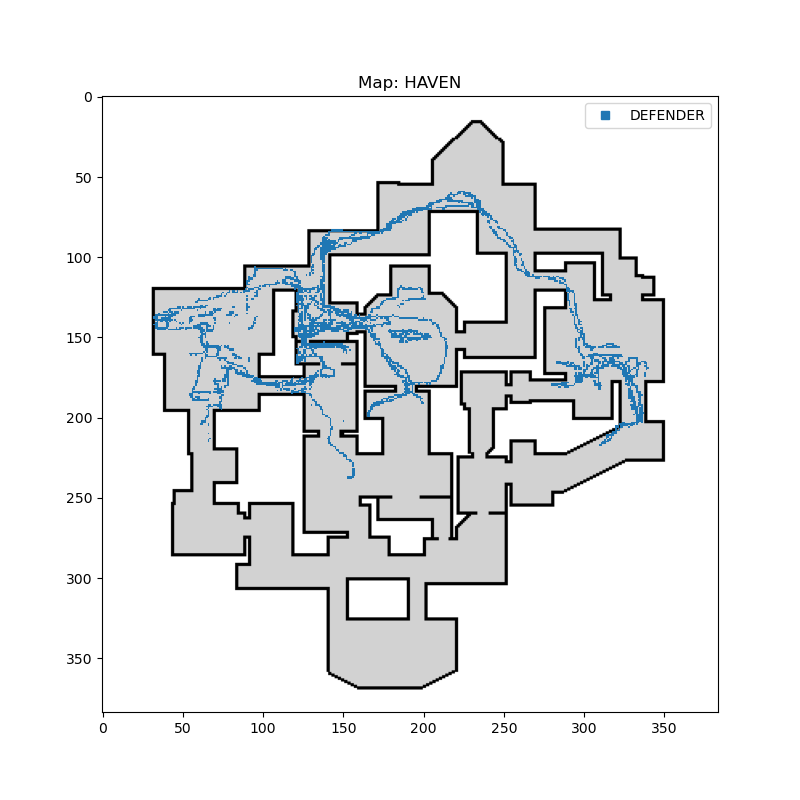
\includegraphics[width=0.8\linewidth]{images/05-output}
	\caption[Output representation as map.]{Output representation as map, summarizing all positions 
	of defender agents during one round on the map "Haven".}
	\label{fig:app:output}
\end{figure}

Image~\ref{fig:intro:minimap} shows different entities that could be possible targets of the detection 
algorithm~(I3). One possibility could be an identification of all players from one team without 
distinguishing the specific agent. The result of such an analysis is shown in 
figure~\ref{fig:app:output}. This graphic summarizes all positions of the defending team during a 
round on the already mentioned map "Haven". In a more advanced approach it is possible to detect 
the specific agents and create motion profiles for each of them. In addition, team or opponent 
abilities could also be recognized. It would be possible as well to combine those detection tasks and 
create various views to present the gathered data. The translation of the data from the video to the 
new representation is done by a neural network (I3). This is trained by the application described in 
section~\ref{subsec:app:trainingapp}. Finally a post-processing algorithm (I4) transforms the output 
data from the neural network into a better recognizable form of presentation (I5).

\subsection{Training Application}\label{subsec:app:trainingapp}

As written in section~\ref{subsec:app:inferenceapp} a trained neural network model is needed to 
transform a Valorant video into another form of representation. This part discusses a concept for an 
application that starts with raw data and outputs a trained machine learning model. That concept is 
outlined in figure~\ref{fig:app:conceptTrain} and differentiates between applications in purple, data 
in blue and programs in green.

For the acquiring of raw data multiple sources are available, in this concept called data platforms. 
An extractor module is intended to obtain the data from those platforms for further usage.
The most intuitive source is the game itself and everything that is rendered on the users screen. In 
that case the extractor is a screen capture device/program that records the screen and outputs a 
video. Other sources are already recorded videos, for example from gamers who upload their 
matches on Youtube for entertainment purposes. But Youtube is not the only platform: as in the 
introduction (Chapter~\ref{chpt:introduction}) mentioned especially during corona pandemic 
streaming platforms like Twitch~\cite{twitch} became popular and there are many creators live 
streaming their Valorant gameplay. So this data could be captured directly while they are streaming 
or afterwards, because the streams are saved to ensure a possibility for people to watch the stream 
after it was broadcasted. In the case of available videos a download script is needed to get the data 
from the platforms.

\begin{figure}
	\centering
	\begin{tikzpicture}[x=0.75pt,y=0.75pt,yscale=-1,xscale=1]
		\draw  [color={rgb, 255:red, 147; green, 25; blue, 212 }  ,draw opacity=1 ][line width=2.25]  
		(250,10) -- (400,10) -- (400,100) -- (250,100) -- cycle ;
		\draw  [color={rgb, 255:red, 147; green, 25; blue, 212 }  ,draw opacity=1 ][line width=2.25]  
		(60,200) -- (590,200) -- (590,540) -- (60,540) -- cycle ;
		\draw  [color={rgb, 255:red, 65; green, 117; blue, 5 }  ,draw opacity=1 ][line width=2.25]  
		(260,130) -- (390,130) -- (390,170) -- (260,170) -- cycle ;
		
		\draw [line width=2.25]    (325,100) -- (325,125) ;
		\draw [shift={(325,130)}, rotate = 270] [fill={rgb, 255:red, 0; green, 0; blue, 0 }  ][line 
		width=0.08]  [draw opacity=0] (11.43,-5.49) -- (0,0) -- (11.43,5.49) -- cycle    ;
		\draw [line width=2.25]    (325,170) -- (325,195) ;
		\draw [shift={(325,200)}, rotate = 270] [fill={rgb, 255:red, 0; green, 0; blue, 0 }  ][line 
		width=0.08]  [draw opacity=0] (11.43,-5.49) -- (0,0) -- (11.43,5.49) -- cycle    ;
		\draw  [color={rgb, 255:red, 74; green, 144; blue, 226 }  ,draw opacity=1 ][line width=2.25]  
		(70,240) -- (220,240) -- (220,330) -- (70,330) -- cycle ;
		\draw  [color={rgb, 255:red, 74; green, 144; blue, 226 }  ,draw opacity=1 ][line width=2.25]  
		(280,50) -- (370,50) -- (370,90) -- (280,90) -- cycle ;
		
		\draw  [color={rgb, 255:red, 65; green, 117; blue, 5 }  ,draw opacity=1 ][line width=2.25]  
		(100,480) -- (290,480) -- (290,520) -- (100,520) -- cycle ;
		
		\draw  [color={rgb, 255:red, 74; green, 144; blue, 226 }  ,draw opacity=1 ][line width=2.25]  
		(250,240) -- (400,240) -- (400,450) -- (250,450) -- cycle ;
		\draw  [color={rgb, 255:red, 49; green, 53; blue, 213 }  ,draw opacity=1 ][line width=1.5]  
		(100,280) -- (190,280) -- (190,310) -- (100,310) -- cycle ;
		\draw  [color={rgb, 255:red, 49; green, 53; blue, 213 }  ,draw opacity=1 ][line width=1.5]  
		(280,280) -- (370,280) -- (370,310) -- (280,310) -- cycle ;
		
		\draw  [color={rgb, 255:red, 49; green, 53; blue, 213 }  ,draw opacity=1 ][line width=1.5]  
		(280,340) -- (370,340) -- (370,370) -- (280,370) -- cycle ;
		
		\draw  [color={rgb, 255:red, 49; green, 53; blue, 213 }  ,draw opacity=1 ][line width=1.5]  
		(280,400) -- (370,400) -- (370,430) -- (280,430) -- cycle ;
		
		\draw [line width=1.5]    (325,310) -- (325,336) ;
		\draw [shift={(325,340)}, rotate = 270] [fill={rgb, 255:red, 0; green, 0; blue, 0 }  ][line 
		width=0.08]  [draw opacity=0] (9.29,-4.46) -- (0,0) -- (9.29,4.46) -- cycle    ;
		\draw [line width=1.5]    (325,370) -- (325,396) ;
		\draw [shift={(325,400)}, rotate = 270] [fill={rgb, 255:red, 0; green, 0; blue, 0 }  ][line 
		width=0.08]  [draw opacity=0] (9.29,-4.46) -- (0,0) -- (9.29,4.46) -- cycle    ;
		\draw [line width=2.25]    (220,280) -- (245,280) ;
		\draw [shift={(250,280)}, rotate = 180] [fill={rgb, 255:red, 0; green, 0; blue, 0 }  ][line 
		width=0.08]  [draw opacity=0] (11.43,-5.49) -- (0,0) -- (11.43,5.49) -- cycle    ;
		\draw  [color={rgb, 255:red, 74; green, 144; blue, 226 }  ,draw opacity=1 ][line width=2.25]  
		(430,240) -- (580,240) -- (580,330) -- (430,330) -- cycle ;
		\draw  [color={rgb, 255:red, 49; green, 53; blue, 213 }  ,draw opacity=1 ][line width=1.5]  
		(460,280) -- (550,280) -- (550,310) -- (460,310) -- cycle ;
		
		\draw [line width=2.25]    (400,280) -- (425,280) ;
		\draw [shift={(430,280)}, rotate = 180] [fill={rgb, 255:red, 0; green, 0; blue, 0 }  ][line 
		width=0.08]  [draw opacity=0] (11.43,-5.49) -- (0,0) -- (11.43,5.49) -- cycle    ;
		\draw  [color={rgb, 255:red, 65; green, 117; blue, 5 }  ,draw opacity=1 ][line width=2.25]  
		(380,480) -- (570,480) -- (570,520) -- (380,520) -- cycle ;
		
		\draw [line width=1.5]  [dash pattern={on 1.69pt off 2.76pt}]  (195,480) -- (195,465) -- 
		(325,465) -- (325,454) ;
		\draw [shift={(325,450)}, rotate = 90] [fill={rgb, 255:red, 0; green, 0; blue, 0 }  ][line 
		width=0.08]  [draw opacity=0] (9.29,-4.46) -- (0,0) -- (9.29,4.46) -- cycle    ;
		\draw [line width=1.5]  [dash pattern={on 1.69pt off 2.76pt}]  (195,465) -- (195,400) -- 
		(145,400) -- (145,334) ;
		\draw [shift={(145,330)}, rotate = 90] [fill={rgb, 255:red, 0; green, 0; blue, 0 }  ][line 
		width=0.08]  [draw opacity=0] (9.29,-4.46) -- (0,0) -- (9.29,4.46) -- cycle    ;
		\draw [line width=1.5]  [dash pattern={on 1.69pt off 2.76pt}]  (475,480) -- (475,400) -- 
		(505,400) -- (505,334) ;
		\draw [shift={(505,330)}, rotate = 90] [fill={rgb, 255:red, 0; green, 0; blue, 0 }  ][line 
		width=0.08]  [draw opacity=0] (9.29,-4.46) -- (0,0) -- (9.29,4.46) -- cycle    ;
		
		\draw (258,16) node [anchor=north west][inner sep=0.75pt]   [align=left] {{\large Data 
		Platform}};
		\draw (68,207) node [anchor=north west][inner sep=0.75pt]   [align=left] {{\large Training 
		Application}};
		\draw (289,64) node [anchor=north west][inner sep=0.75pt]   [align=left] {RAW Data};
		\draw (294,143) node [anchor=north west][inner sep=0.75pt]   [align=left] {Extractor};
		\draw (79,251) node [anchor=north west][inner sep=0.75pt]   [align=left] {RAW Data};
		\draw (259,251) node [anchor=north west][inner sep=0.75pt]   [align=left] {INTERIM Data};
		\draw (439,251) node [anchor=north west][inner sep=0.75pt]   [align=left] {PROCESSED Data};
		\draw (392,492) node [anchor=north west][inner sep=0.75pt]   [align=left] {Machine Learning 
		Model};
		\draw (116,288) node [anchor=north west][inner sep=0.75pt]   [align=left] {VIDEOS};
		\draw (471,288) node [anchor=north west][inner sep=0.75pt]   [align=left] {DATASET};
		\draw (293,288) node [anchor=north west][inner sep=0.75pt]   [align=left] {FRAMES};
		\draw (298,348) node [anchor=north west][inner sep=0.75pt]   [align=left] {CROPS};
		\draw (296,408) node [anchor=north west][inner sep=0.75pt]   [align=left] {LABELS};
		\draw (125,492) node [anchor=north west][inner sep=0.75pt]   [align=left] {Data 
		Pre-Processing};
	\end{tikzpicture}
	\caption{Concept for the training application.}
	\label{fig:app:conceptTrain}
\end{figure}

In the training application the acquired raw data is available in video format. In order to train a neural 
network several pre-processing steps are necessary to transform the raw data into a usable dataset. 
Therefore a data pre-processing component has to be built. The task of this module is to separate 
the video into individual frames, crop the frames onto the minimap, label the created images of the 
minimap and build a dataset. The pictures of the cropped minimap are reffered to as crops in the 
context of this project's implementation and in image~\ref{fig:app:conceptTrain}.

The first step of splitting the video into frames has to be done, because the neural network is 
trained with images even though inference is done on videos. The reason is that the annotation of 
images is easier than with videos. As noted in section~\ref{subsec:app:inferenceapp} the information 
from the minimap is sufficient and therefore the frames become cropped onto the minimap. That 
results in significant smaller images, which need less memory and a lot of irrelevant and disturbing 
information is discarded. Annotations describing where detectable entities are in the image are 
created in the labeling step. These labels are used by the neural network as ground truth 
during training. Finally the crops and the labels are combined into a dataset that can be used by the 
machine learning model.

\section{Data}\label{sec:app:data}

This section describes the data that is actually used to carry out this project. Twitch serves as the 
data platform and a video~\cite{valVideo2023} of professionals playing at the Valorant 
Champions Tour 2023 in Los Angeles was downloaded. The chosen part of the video shows a match 
between the European team FNATIC and the American team LOUD. They played on three different 
maps (Ascent, Haven and Split). The video was downloaded with the tool yt-dlp~\cite{ytdlp2023} 
and the download script~\ref{lst:app:download}. 

\begin{minipage}{\linewidth}
	\vspace*{0.5cm}
	\begin{lstlisting}[language=Bash, keywordstyle=\color{black}, 
		caption=Download script to get the raw data., label=lst:app:download]
		#!/bin/bash
		
		s="$1"		# start timestamp
		e="$2"		# end timestamp
		n="$3"		# output name
		
		yt-dlp --external-downloader ffmpeg --external-downloader-args 
		"ffmpeg_i:-ss "$s".00 -to "$e".00" --output ""$n".mp4" 
		https://www.twitch.tv/videos/1907425469
	\end{lstlisting}
\end{minipage}

That script gets a start and an end timestamp and downloads the specified sequence of the selected 
video. With that technique the original video became downloaded without replays and 
non-gameplay. Consistent with the requirements the match was simultaneously split into single 
rounds. Therefore raw gameplay of three maps is available for further use within the project.

\begin{figure}
	\centering
	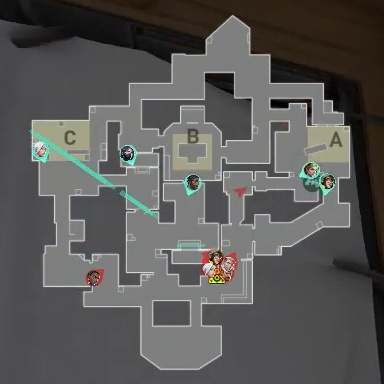
\includegraphics[width=0.7\linewidth]{images/06-input}
	\caption[Cropped input data.]{Cropped input data from the map "Haven".}
	\label{fig:app:input}
\end{figure}

The downloaded sequences show a different screen than depicted so far. The reason is that 
this video was part of the official sports reporting and therefore it is from observer view. The 
difference can be seen in figure~\ref{fig:app:input}. From players perspective only the agents of the 
same team and some enemy abilities can be seen on the minimap (see 
image~\ref{fig:intro:minimap}) but the opponents positions stay hidden. In contrast for spectators all 
players are visible on the map. That is advantageous for the learning task, because with that data the 
view of attackers and defenders can be trained at once. 

\section{YOLOv5}\label{sec:app:yolov5}

As machine learning model YOLOv5~\cite{jocher2020} was chosen because the usability of 
Ultralytics version is very good and feasibility already was proven. In addition, it is open source and 
continues to be actively developed~\cite{terven2023, river2021}. Furthermore with YOLOv5 
pre-trained checkpoints can be used for transfer learning~\cite{jocher2020}.

YOLOv5 is the first version that uses PyTorch~\cite{pytorch} instead of Darknet~\cite{darknet13} as 
machine learning framework in the YOLO series. Both of them are open source and Darknet was 
developed by Joseph Redmon the first author of "You Only Look Once". While Darknet is 
written in C and CUDA, PyTorch uses Python and makes training and testing easier for customized 
datasets~\cite{darknet13, pytorch, aydin2023, terven2023}. The architecture of YOLOv5 is divided 
into three parts: backbone, neck and head~\cite{archYolov5}. That is a common architecture for 
object detectors~\cite{terven2023}. 

In general the backbone is used to extract features from the input image and that is done with a 
\gls{acr-cnn}. Thereby earlier layers extract low-level features like edges and textures and deeper 
layers are used for detection of higher-level entities (object parts and semantic information). The 
neck connects the backbone and the head with additional convolutional layers, a \gls{acr-fpn} or 
other components that improve the feature representations from the backbone. While the goal of 
the backbone is to capture features at different scales the focus of the neck is to enhance the spatial 
and semantic information across those different scales. The head makes the actual predictions on 
the provided features and mostly consists of several task-specific subnetworks for localization and 
classification. Predictions are made for each object candidate and in a post-processing step only the 
most confident detections are kept. A possible algorithm to filter out overlapping predictions is 
\gls{acr-nms}~\cite{terven2023}.

The backbone of YOLOv5 is a modified CSPDarknet53 a \gls{acr-cnn} with 53 convolutional 
layers~\cite{terven2023, redmon2018, wang2020}. It starts with a  layer with a large window size 
(called stem) and has the goal to reduce memory and computational costs. Further each 
convolutional block consists of a convolutional layer followed by \gls{acr-bn} and a \gls{acr-silu} 
activation. The neck contains a \gls{acr-sppf} layer that processes the features at different scales 
and intends to speed up computation by pooling the different scaled features into a fixed-size 
feature map. Afterwards upsample layers increase the resolution of those feature 
maps~\cite{terven2023}. The complete architecture of YOLOv5 is depicted in 
figure~\ref{fig:aa:archyolov5}.

As mentioned before \gls{acr-nms} is a post-processing algorithm, with the goal to reduce the 
number of overlapping predictions. The neural network generates so called bounding boxes during 
detection, to describe the location and size of an object~\cite{anchor2023}, but typically it is 
generating multiple boxes per entity and each bounding box has a different confidence score. 
\GLS{acr-nms} is used to filter out irrelevant bounding boxes by keeping just the most accurate per 
object. Therefore an \gls{acr-iou} and confidence threshold is defined for 
inference~\cite{terven2023}.

For training YOLOv5 can use data augmentation techniques, helping to improve the generalization 
ability and to reduce overfitting. The following two were used to train the experiments described in 
chapter~\ref{chpt:evaluation}. The first technique is called mosaic augmentation and thereby 
multiple images are combined into a large image with the goal to improve the handling of different 
object scales and translations. The second one is called HSV augmentation and randomly changes 
hue, saturation and value of the images and therefore creates a bigger variance in the learned 
data~\cite{archYolov5}.

Finally the training strategy AutoAnchor has to be described. This is an algorithm developed by 
Ultralytics~\cite{terven2023, archYolov5}. The training of YOLOv5 is based on anchor boxes with 
aim on improving the prediction quality. Later versions of YOLO did not need anchor boxes 
anymore~\cite{terven2023, zheng2022}. As mentioned before, the predictions of objects are based 
on bounding boxes, but unfortunately the objects have different shapes and sizes and so the boxes 
must have those too. For that so called anchors are used which are building a predefined set of 
bounding boxes with different shapes and sizes. The detection algorithm then has to decide which 
anchor matches best~\cite{anchor2023}. Ultralytics AutoAnchor algorithm is a pre-training tool that 
adjusts the predefined anchor boxes to better fit the ground truth boxes of custom 
datasets~\cite{terven2023, archYolov5}.

\section{Implementation}\label{sec:app:impl}

This section gives an overview of the realization of this project, starting from the point that the raw 
data is available as multiple videos showing single rounds of the game Valorant. The objective of this 
project was to carry out a machine learning project as realistic as possible. Due to that an 
application scenario was defined: the creation of an application that is capable to analyze gameplay 
of the video game Valorant. On this scenario the goal was to start with acquiring and pre-processing 
of data, training a machine learning model and post-process the output. An important intention was 
trying to use an already existing model and apply training, evaluation and inference on that, instead 
of implementing a preformed architecture. The reason is that the existing learning framework can 
provide pre-trained weights that can be used for transfer learning. Especially for the backbone it is 
good to be trained on a large-scale image classification task~\cite{terven2023} and that is not 
efficiently possible on a performance limited private GPU. Therefore it is interesting to compare the 
performance of a learning task form scratch with one using transfer learning (see 
chapter~\ref{chpt:evaluation}).

The first big task was the pre-processing of the data. As mentioned in the concept, labeling of 
images is easier than on videos. Since YOLOv5 can be trained on pictures and afterwards applied on 
videos, images as training data were created. Therefore several python scripts were implemented 
that split the videos into single frames (one per second) and than crop them to the minimap. Those 
steps result in images like the one depicted in figure~\ref{fig:app:input} with a resolution of 384 by 
384 pixels. After that labels had to be created manually, which then can serve as ground truth for 
the training. For this purpose the open source labeling tool "Label Studio"~\cite{labelstudio} was 
used.

\subsection{Label Studio}\label{subsec:app:labelstudio}

Label Studio is a web application that can be hosted by yourself. It can be installed via python and 
the server runs locally in the simplest configuration. In a first step Label Studio has to be initialized 
and a user must be created. Following a new project for the labeling task can be set up via the web 
interface. It is possible to reference the local images and configure the labels. As labeling is very 
time consuming, only a distinction between attackers and defenders was made in this project. In 
figure~\ref{fig:app:labelstudio} the labeling interface of Label Studio is depicted. As it can be seen,  
circular labels were used, because with them it was easy to set a point into the middle of each 
agent. Initially it was planned to label the images of all three available maps. This turned out to be a 
very time-consuming process, although a single label could be created very fast with the used 
settings. Therefore only 1000 images of the map "Ascent" were labeled and it only was possible to 
train the neural network with this data. When labeling was finished the labels were exported in XML 
format. That file contains information about the position of all objects and their assigned class for 
each image.

\begin{figure}
	\centering
	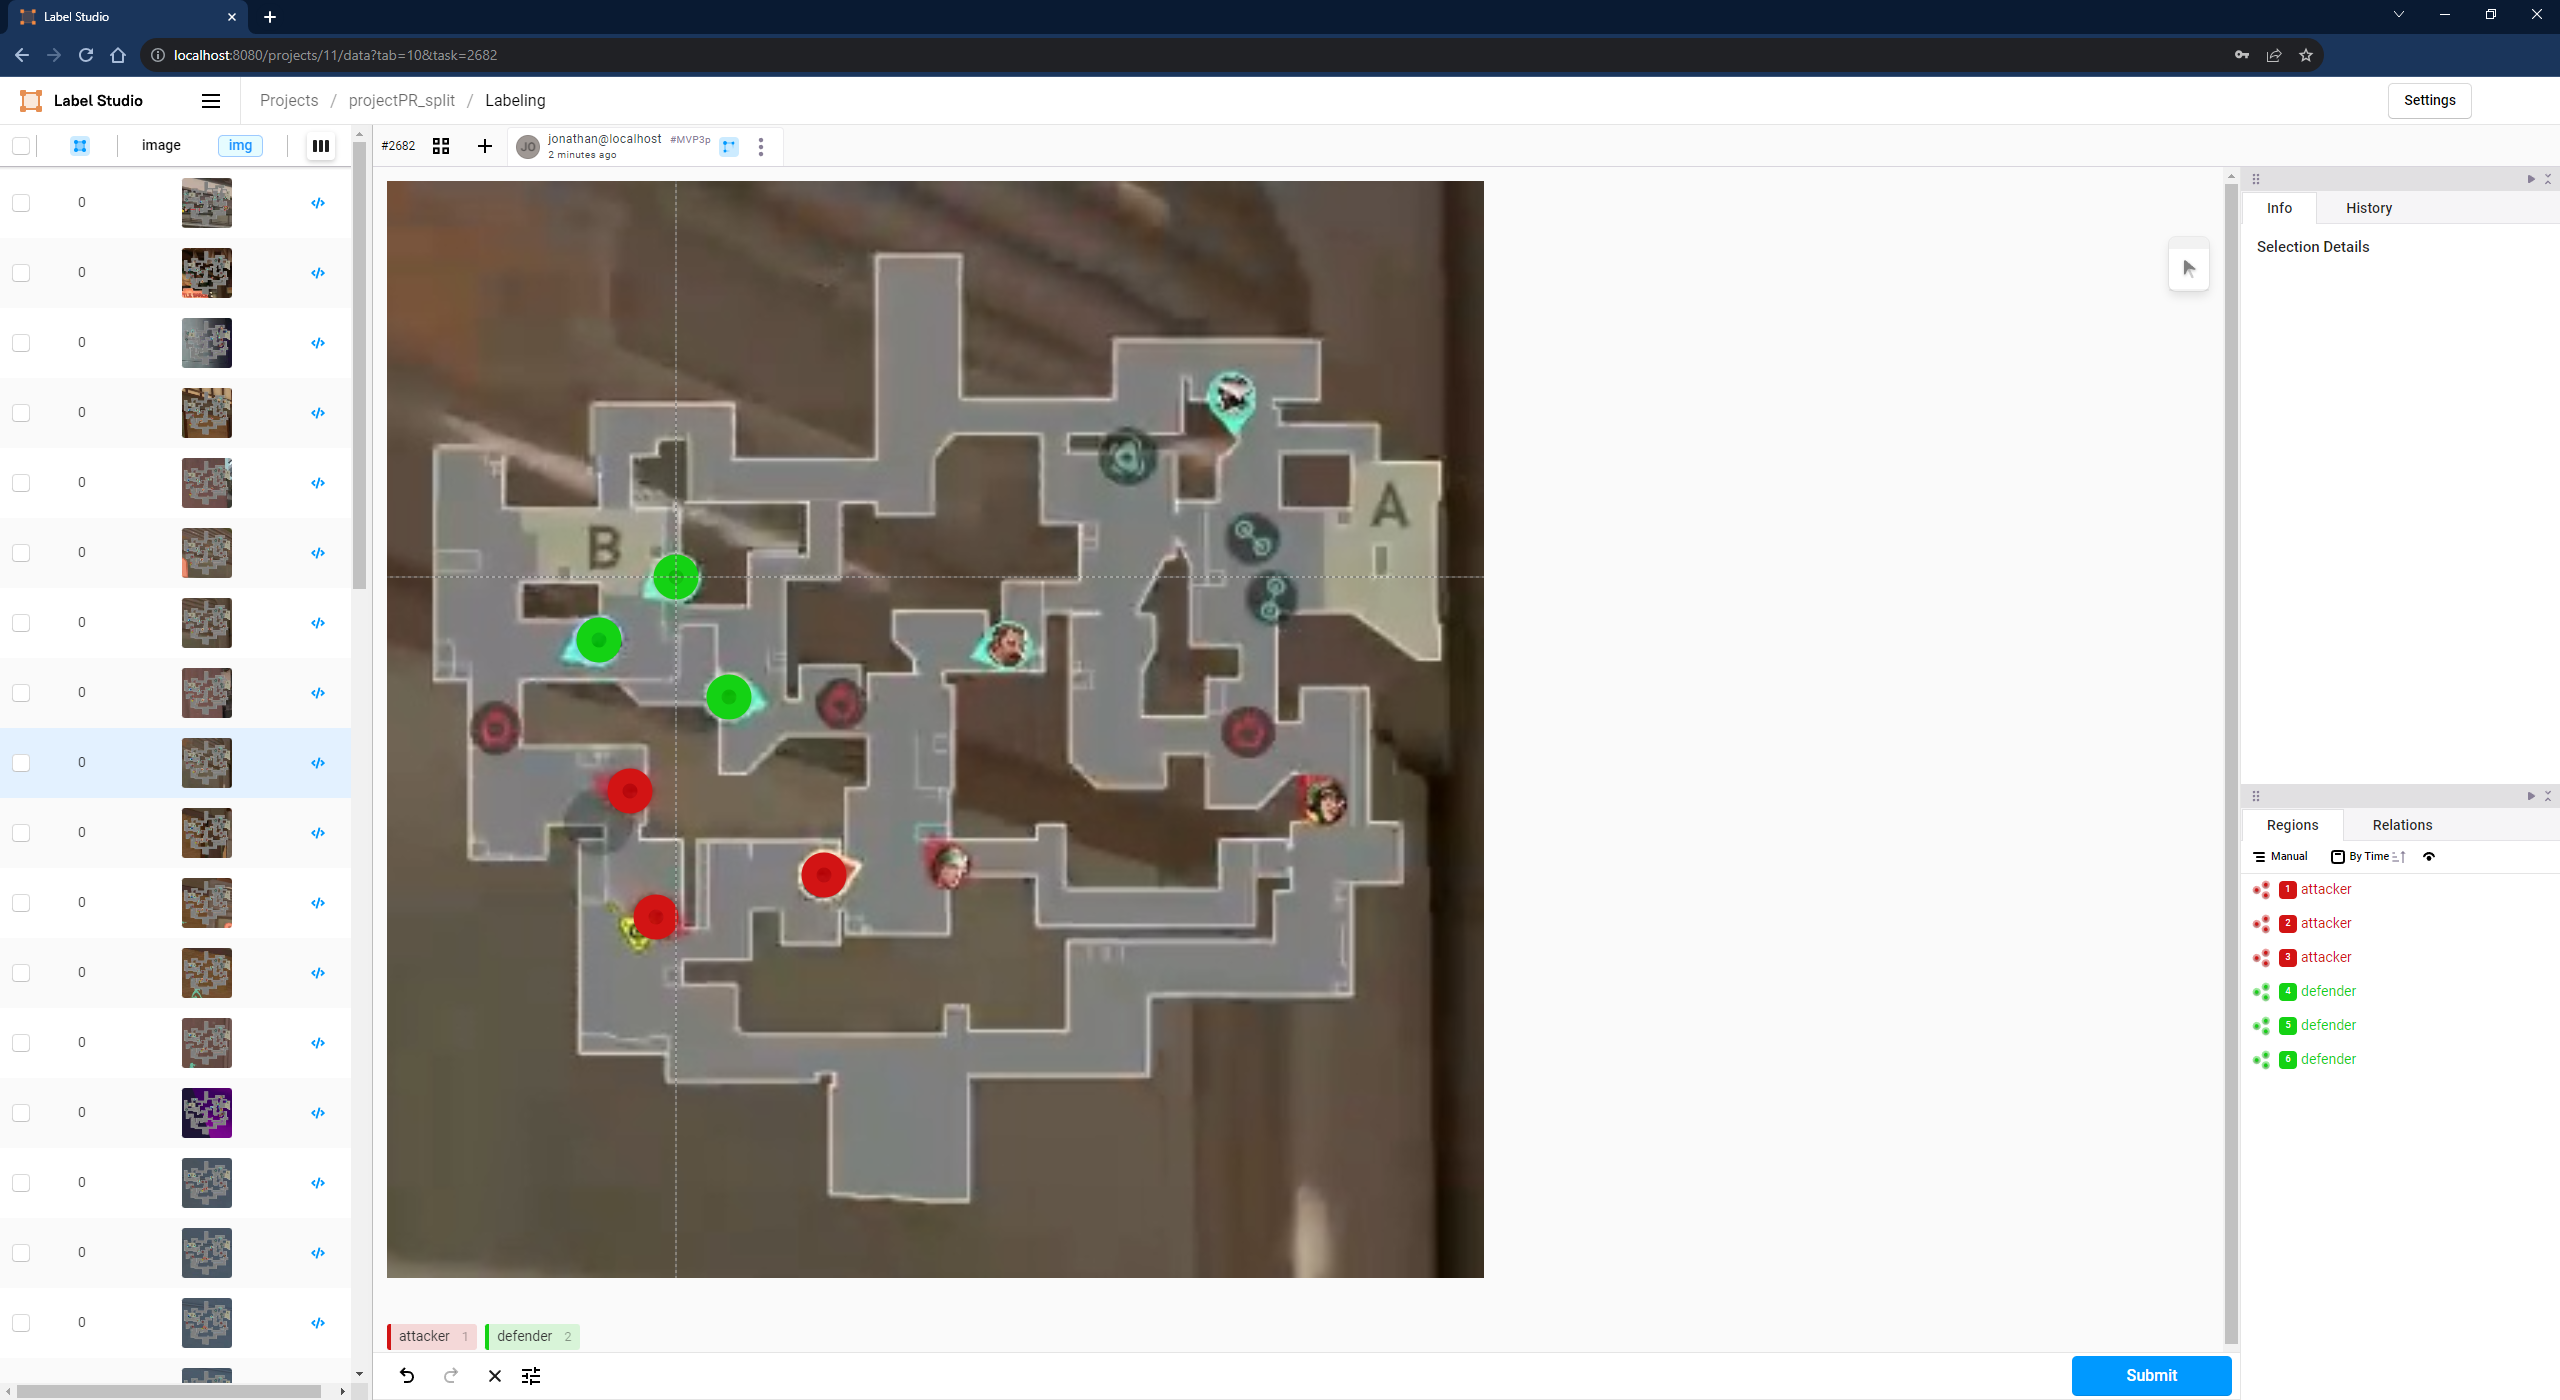
\includegraphics[width=0.95\linewidth]{images/07-labelstudio}
	\caption[Interface of Label Studio.]{Labeling interface of Label Studio with partially labeled 
	attackers (red) and defenders (green).}
	\label{fig:app:labelstudio}
\end{figure}

\subsection{Dataset}\label{subsec:app:dataset}

After labeling, the images and labels had to be combined into a dataset that can be used by 
YOLOv5. The learning framework YOLO comes with its own dataset format and for that reason a 
parser was implemented to create an appropriate dataset. Since the used neural network creates 
bounding boxes it is necessary that ground truth also contains those boxes but so far only the 
centers of the objects were labeled. 

In YOLO format one file is created for every image and this file contains one line per object with the 
following information~\cite{yoloLabels}:

\begin{itemize}
	\item class label
	\item $x$ center of the object
	\item $y$ center of the object
	\item width of the bounding box
	\item height of the bounding box
\end{itemize}

Advantageous is that the class label as well as the $x$ and $y$ centers of the object already are 
available and that every agent on the minimap has the same size. Therefore one default size of the 
bounding box can be used to bring the labels into YOLO format and build the dataset. Thereby the 
train/validation/test split already has to be specified. In this project 80~\% of the data was used for 
training and always 10~\% for validation and testing.

\subsection{Training}\label{subsec:app:training}

This section describes how YOLOv5 can be trained with a custom dataset. First of all a separate 
python environment is recommended and YOLO has to be downloaded from 
GitHub\footnote{\url{https://github.com/ultralytics/yolov5}}.  In the repository a requirements file can 
be found and it is necessary to install all listed packages. Per default a CPU version of PyTorch is 
installed, if a GPU is available the appropriate version has to be switched. This project was 
implemented on a Windows computer with a NVIDIA GeForce GTX 1660 SUPER with 6 GB graphics 
memory. This setup was not compatible with the latest version of PyTorch and CUDA. Therefore 
Python 3.9 and PyTorch 1.10.1 with CUDA 10.2 had to be installed.

After completing the installation YOLOv5 is ready for usage. A Python script starting the training is 
available in the root folder of the repository and a general call of the script is specified in 
instruction~\ref{lst:app:traincmd}. 

Besides the number of epochs and the batch size the path to a configuration file inside the used 
dataset has to be specified (line 10). The project path (line 11) describes the target folder where all 
output files of the training runs are saved. Additionally the image size is set to 384 pixels because of 
the resolution of the cropped maps and the optimizer SGD is a default setting of YOLOv5. 
Furthermore data is cached in the RAM instead of the disk what speeds up training and as device the 
available GPU is chosen. Finally the weights of the network are saved every 10 epochs.

\renewcommand{\lstlistingname}{Instruction}
\begin{minipage}{\linewidth}
	\vspace*{0.5cm}
	\begin{lstlisting}[language=Bash, keywordstyle=\color{black}, 
		caption=General command to start the training of YOLOv5., label=lst:app:traincmd]
		python train.py
		
			--epochs <NUM_EPOCHS>
			--batch-size <BATCH_SIZE>
			
			--weights yolov5s.pt
			--img 384
			--optimizer SGD
			
			--data <PATH_TO_DATASET>.yaml
			--project <PATH_TO_PROJECT>
			--name train
			
			--cache ram
			--device cuda:0
			--save-period 10
	\end{lstlisting}
\end{minipage}

If transfer learning is used or training starts from scratch is decided by specifying \texttt{weights} 
for the network. In the case of instruction~\ref{lst:app:traincmd} transfer learning is applied. YOLOv5 
is published in five scaled versions, with different width and depth of the convolutional modules. 
They were created that YOLOv5 can be used with different hardware 
requirements~\cite{jocher2020, terven2023}. In this project the second smallest version was chosen 
and is specified by \texttt{yolov5s.pt}, with \texttt{s} for small. This is a lightweight model for 
low-resource devices~\cite{terven2023}. Those weights are trained for 80 classes on the Microsoft 
COCO (Common Objects in Context) dataset~\cite{lin2014, jocher2020}. For training from scratch 
the specification of the \texttt{weights} must be let empty and a network configuration file has to be 
provided. This file defines the structure of the network as well as the weights file does.

A special option for transfer learning is the \texttt{freeze} command. With that a number of 
layers are not trained. As mentioned at the beginning of section~\ref{sec:app:impl}, it makes sense 
to train the backbone on a large-scale image classification task such as the COCO dataset. In order 
to save computation costs the already pre-trained backbone weights can be frozen and only the rest 
of the network is trained on the new data~\cite{y5TransfLearn}. Additionally after training without 
backbone all weights can be fine tuned in a second learning task using a small learning rate. 
Therefore instead of the downloaded weights those from the first training step are used.

Just like the training script there is also one for validation that can be executed on the validation and 
test data. Which data are used can be specified by the \texttt{task} option. A general version of the 
commands are given in the appendix (see instructions~\ref{lst:aa:valcmd} and~\ref{lst:aa:testcmd}).

\subsection{Inference}\label{subsec:app:inference}

Last but not least there is also a script for the detection task. The appropriate command is 
specified in instruction~\ref{lst:app:inferencecmd}. This script can be applied on images as well as 
on videos and the file can be specified with the \texttt{source} option. Further, it is possible to define 
a confidence threshold and an \gls{acr-iou} threshold. As mentioned in section~\ref{sec:app:yolov5} 
the \gls{acr-nms} algorithm uses those thresholds to filter out irrelevant bounding boxes and thereby 
improves detection quality. 

\begin{minipage}{\linewidth}
	\vspace*{0.3cm}
	\begin{lstlisting}[language=Bash, keywordstyle=\color{black}, 
		caption=General command to start the detection with YOLOv5., label=lst:app:inferencecmd]
		python detect.py
		
			--weights <PATH_TO_PROJECT>/train/weights/best.pt
			
			--source <PATH_TO_DATA>
			--project <PATH_TO_PROJECT>/detect
			--name <NAME_OF_DETECT_TASK>
			
			--conf-thres <CONF_THRESH>
			--iou-thres <IOU_THRESH>
			
			--hide-labels
			--save-txt
			--save-conf
						
			--device cuda:0
	\end{lstlisting}
\end{minipage}

The output of the detection script is a folder with one file per image containing the detected objects. 
That file has the same structure as the files of the labels. Additionally an image or a video is 
created by the script, showing the inferred bounding boxes. Based on the detected objects a graphic 
can be derived that summarizes all positions of a team in one round. A script has been implemented 
for this and an output example is shown in figure~\ref{fig:app:output}.

\chapter{Evaluation}\label{chpt:evaluation}
\glsresetall

In order to test the application two neural networks were trained and evaluated. In this chapter the 
training settings as wall as the results of the evaluation and the detection tests are discussed.

\section{Experiments}\label{sec:eval:experiments}

Both neural networks were trained on a dataset containing 1000 labeled images of the map 
"Ascent". The dataset has a train/validation/test split as described in 
section~\ref{subsec:app:dataset}. In each case 600 epochs and a batch size of 64 images were 
used. That is the highest possible batch size due to limited graphics memory of the used GPU. As 
network architecture the small version (\texttt{yolov5s}) of the YOLOv5 model was deployed.

The first neural network (Model 1) was trained using the transfer learning concept. Starting 
point were the weights of the pre-trained \texttt{yolov5s} model. As described in 
section~\ref{subsec:app:training} the \texttt{freeze} option was applied to deactivate the adaptation 
of the backbone. Using the small YOLOv5 model ten layer had to be frozen. The number of 
backbone layers can be found in the network configuration file in the YOLOv5 
repository~\cite{jocher2020}. With this approach the training of the backbone only is done on the 
COCO dataset and so a huge part of the network is not refined on the actual data. Therefore a fine 
tuning task is applied, that trains the whole network for additional 100 epochs. In order to prevent 
major adjustments special fine tuning parameters including a small learning rate are used. The 
applied hyper parameters were defined by Ultralytics.

The second network (Model 2) serves as point of reference and was trained from scratch. Thereby it 
is necessary to provide a network configuration for the training script. That was done by using the 
configuration file of the \texttt{yolov5s} model and adapting the number of trained classes. In this 
case there are two classes (attacker and defender).

\section{Results}\label{sec:eval:results}

\begin{table}
	\centering
	\captionabove[Summary of metric results for the best epochs.]{Overview of metric results for the 
	weights from the best epoch.}
	\label{tab:eval:metricResultsBest}
	\begin{tabular}{p{0.03\textwidth}p{0.16\textwidth}p{0.02\textwidth}p{0.13\textwidth}p{0.03\textwidth}S[table-format=3.5]S[table-format=3.5]S[table-format=3.5]}
		\toprule
		&  \multicolumn{1}{c}{Training task} &&  \multicolumn{1}{c}{Epoch} && 
		\multicolumn{1}{c}{$mAP_{50}$} & 	\multicolumn{1}{c}{$mAP_{50-95}$} & 
		\multicolumn{1}{c}{$F1$}\\
		\midrule
		%
		\multicolumn{8}{l}{\bfseries{Model 1, Validation data}} \\[7pt]
		&  \multicolumn{1}{c}{\textsc{train}} &&  \multicolumn{1}{c}{\textsc{best}} && 0.988 & 0.664 & 
		0.978\\[5pt]
		&  \multicolumn{1}{c}{\textsc{finetune}} &&  \multicolumn{1}{c}{\textsc{best}} && 0.995 & 0.825 
		& 0.99\\[7pt]
		%
		\multicolumn{8}{l}{\bfseries{Model 1, Test data}} \\[7pt]
		&  \multicolumn{1}{c}{\textsc{train}} &&  \multicolumn{1}{c}{\textsc{best}} && 0.991 & 0.661 & 
		0.975\\[5pt]
		&  \multicolumn{1}{c}{\textsc{finetune}} &&  \multicolumn{1}{c}{\textsc{best}} && 0.994 & 0.819 
		& 0.986\\[7pt]
		%
		\multicolumn{8}{l}{\bfseries{Model 2, Validation data}} \\[7pt]
		&  \multicolumn{1}{c}{\textsc{train}} &&  \multicolumn{1}{c}{\textsc{best}} && 0.993 & 0.682 & 
		0.988\\[7pt]
		%
		\multicolumn{8}{l}{\bfseries{Model 2, Test data}} \\[7pt]
		&  \multicolumn{1}{c}{\textsc{train}} &&  \multicolumn{1}{c}{\textsc{best}} && 0.991 & 0.676 & 
		0.986\\
		%
		\bottomrule
	\end{tabular}
\end{table}

First of all the implementation of the concept worked and the whole data pipeline from input video to 
output representation can be applied. The training task of the first model stopped automatically after 
568 epochs because the best results were achieved in epoch 467 and in the following 100 epochs 
no further progress was made. This training task took around 2 hours and fine tuning was done in 45 
minutes. In comparison to that training from scratch is more time-consuming: the network 
needed 4 hours and 20 minutes to complete the training of all 600 epochs. With regard to the time, 
transfer learning gives an advantage.

During training several configurations of the network weights are stored and in the end the training 
script additionally saves the best one in a separate file. The results of the metrics introduced in 
section~\ref{subsec:intro:metrics} for the best configurations are listed in 
table~\ref{tab:eval:metricResultsBest}. The $F1$ score was calculated manually from precision 
and recall. All raw data that were recorded by the evaluation script are appended at the end of this 
report as an extended table containing data of several epochs (Table~\ref{tab:ea:metricResults}). 
For the first model a distinction between the transfer learning task and the fine tuning is made in this 
data and all configurations are evaluated on the validation and on the test split. 

The evaluation of the mean average precision ($mAP$) and the $F1$ score show that the fine tuning 
task of the first model is recommended because of a significant improvement of the performance. 
Considering only the $F1$ score depending on the data split the first model performs better than the 
model that was trained from scratch or they are equal. But relating to the $mAP_{50-95}$ the fine 
tuned model works best.

Therefore the best epoch of the fine tuned neural network was used to perform the detection tasks. 
The confidence and IoU threshold of the \gls{acr-nms} algorithm were set to respectively 0.7 during 
inference. In figure~\ref{fig:ea:outDetect} the result of an image from the map "Ascent" is shown. 
That image is not part of the used dataset and the bounding boxes were generated by the neural 
network with confidence values between 0.852 and 0.901. In a second step the model was fed with 
videos, starting with the trained map "Ascent". This worked very well, so also a recording of the map 
"Haven" was tested. The network has never learned about the map "Haven" before but the results 
are quite good. They are depicted in the figures~\ref{fig:app:output}, \ref{fig:ea:outputAtt} and 
\ref{fig:ea:outputComb}. This is a satisfying result because it shows a good generalization ability of 
the neural network. Challenging for the model is that the video of "Haven" shows a new background 
and there are other agents in the video with different images. Despite the good results especially in 
the image of the attackers (see figure~\ref{fig:ea:outputAtt}) false predictions in form of single 
fragments at odd places can be seen but that could be improved with additional training on this map.

\chapter{Conclusion and Future Work}\label{chpt:conclusion+future}
\glsresetall

Finally a summary is provided and further ideas to extend the project work is given in the 
\autoref{sec:future} \nameref{sec:future}.

\section{Conclusion}\label{sec:conclusion}

\section{Future Work}\label{sec:future}


\appendix
\chapter{Additions to the application}\label{chpt:applicationAdditions}
\glsresetall

\section{Architecture of Yolov5}\label{sec:aa:archyolov5}

\begin{figure}[H]
	\centering
	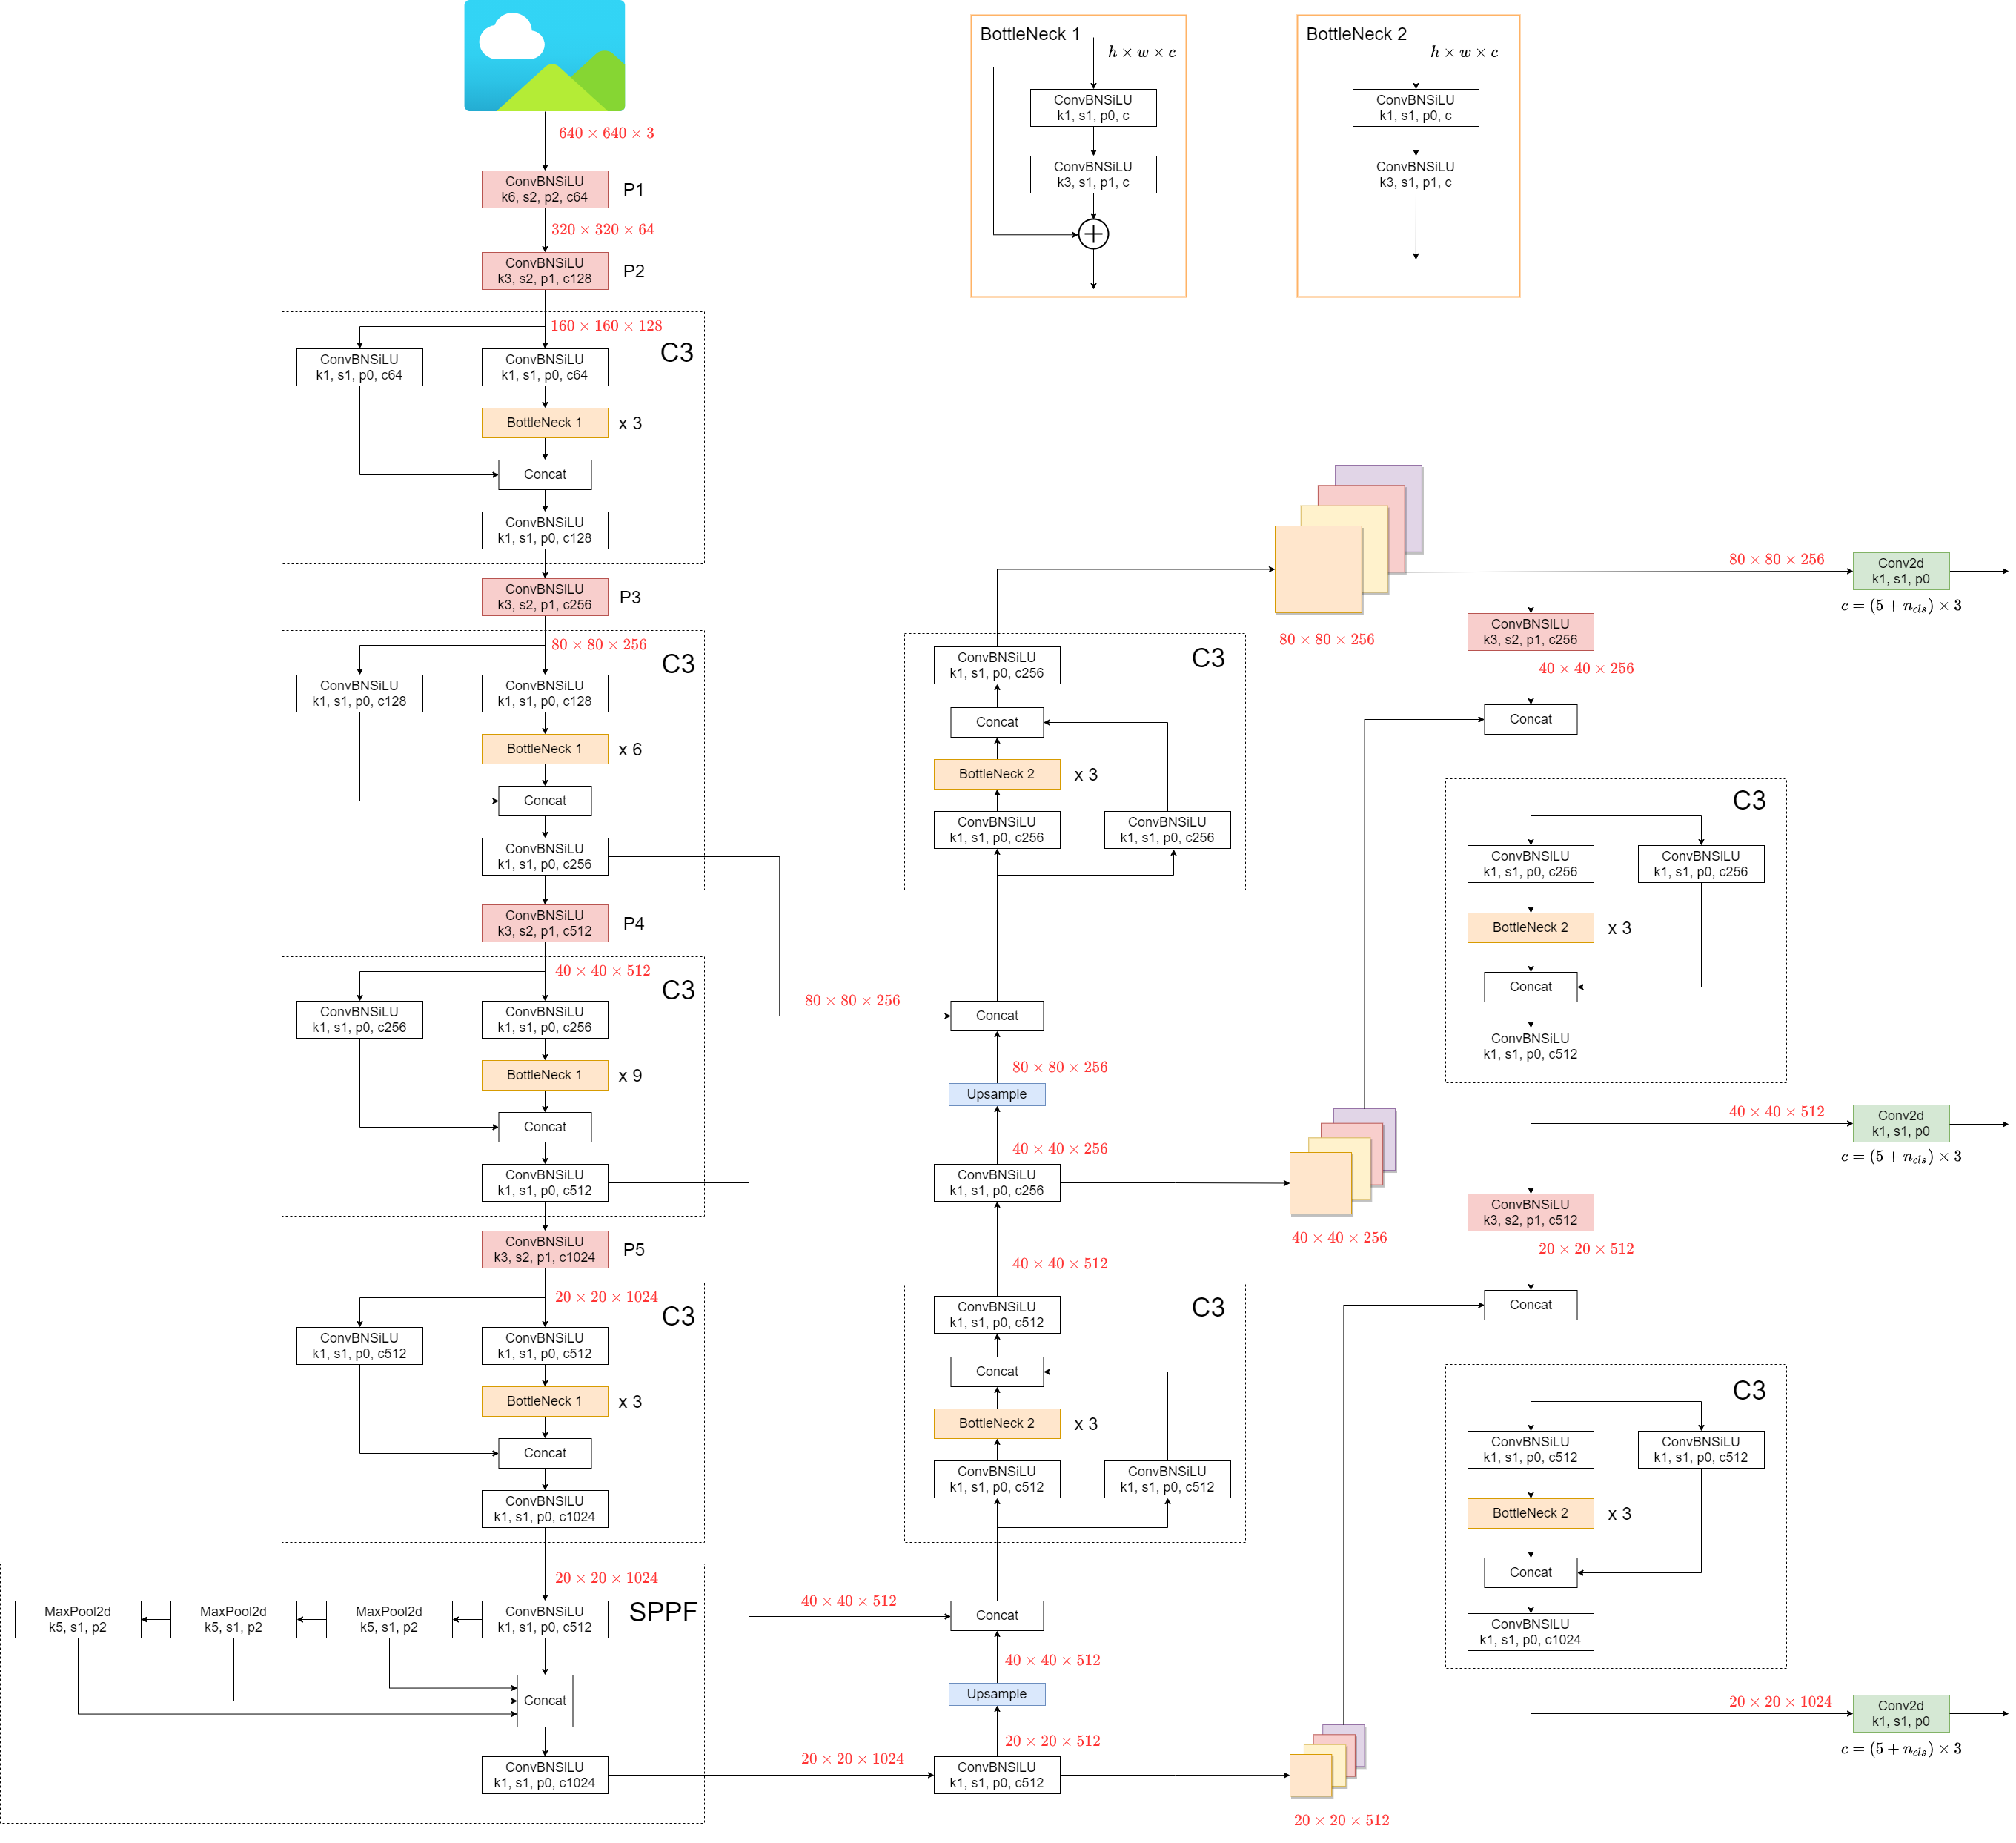
\includegraphics[width=1.0\linewidth]{images/a01-arch-yolov5}
	\caption[Architecture of YOLOv5.]{Architecture of YOLOv5~\cite{archYolov5}.}
	\label{fig:aa:archyolov5}
\end{figure}


\chapter{Additions to the evaluation}\label{chpt:evaluationAdditions}
\glsresetall

\section{Training metrics}\label{sec:ea:trainingMetrics}

\begin{table}[H]
	\centering
	\captionabove[Overview of all metric results.]{Overview of metric results for different training tasks and data splits.}
	\label{tab:ea:metricResults}
	\begin{tabular}{p{0.03\textwidth}p{0.17\textwidth}p{0.03\textwidth}p{0.14\textwidth}p{0.03\textwidth}S[table-format=1.3]S[table-format=1.3]S[table-format=1.3]S[table-format=1.4]}
		\toprule
		&  \multicolumn{1}{c}{Training task} &&  \multicolumn{1}{c}{Epoch} && \multicolumn{1}{c}{$P$} & \multicolumn{1}{c}{$R$} & \multicolumn{1}{c}{$mAP_{50}$} & \multicolumn{1}{c}{$mAP_{50-95}$} \\
		\midrule
		%
		\multicolumn{9}{l}{\bfseries{Model 1, Validation data}} \\[7pt]
		%
		&  \multicolumn{1}{c}{\textsc{train}} &&  \multicolumn{1}{c}{\textsc{best}} && 0.982 & 0.974 & 0.988 & 0.664 \\[5pt]
		&  \multicolumn{1}{c}{\textsc{finetune}} &&  \multicolumn{1}{c}{\textsc{best}} && 0.993 & 0.988 & 0.995 & 0.825 \\[7pt]
		%
		\multicolumn{9}{l}{\bfseries{Model 1, Test data}} \\[7pt]
		%
		&  \multicolumn{1}{c}{\textsc{train}} &&  \multicolumn{1}{c}{\textsc{best}} && 0.974 & 0.977 & 0.991 & 0.661 \\[5pt]
		&  \multicolumn{1}{c}{\textsc{finetune}} &&  \multicolumn{1}{c}{\textsc{best}} && 0.981 & 0.991 & 0.994 & 0.819 \\[7pt]
		%
		\multicolumn{9}{l}{\bfseries{Model 2, Validation data}} \\[7pt]
		%
		&  \multicolumn{1}{c}{\textsc{train}} &&  \multicolumn{1}{c}{\textsc{best}} && 0.985 & 0.992 & 0.993 & 0.682 \\[7pt]
		%
		\multicolumn{9}{l}{\bfseries{Model 2, Test data}} \\[7pt]
		%
		&  \multicolumn{1}{c}{\textsc{train}} &&  \multicolumn{1}{c}{\textsc{best}} &&  0.983 & 0.99  & 0.991 & 0.676 \\
		%
		\bottomrule
	\end{tabular}
\end{table}

\newpage

\section{Inference results}\label{sec:ea:inferenceResults}

\begin{figure}[H]
	\centering
	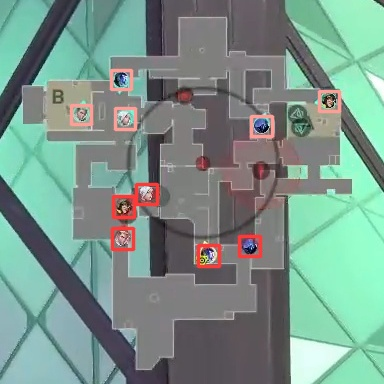
\includegraphics[width=0.8\linewidth]{images/a02-detect}
	\caption[Detected bounding boxes.]{Detected bounding boxes for a not trained image from the map "Ascent".}
	\label{fig:ea:outDetect}
\end{figure}

\begin{figure}[H]
	\centering
	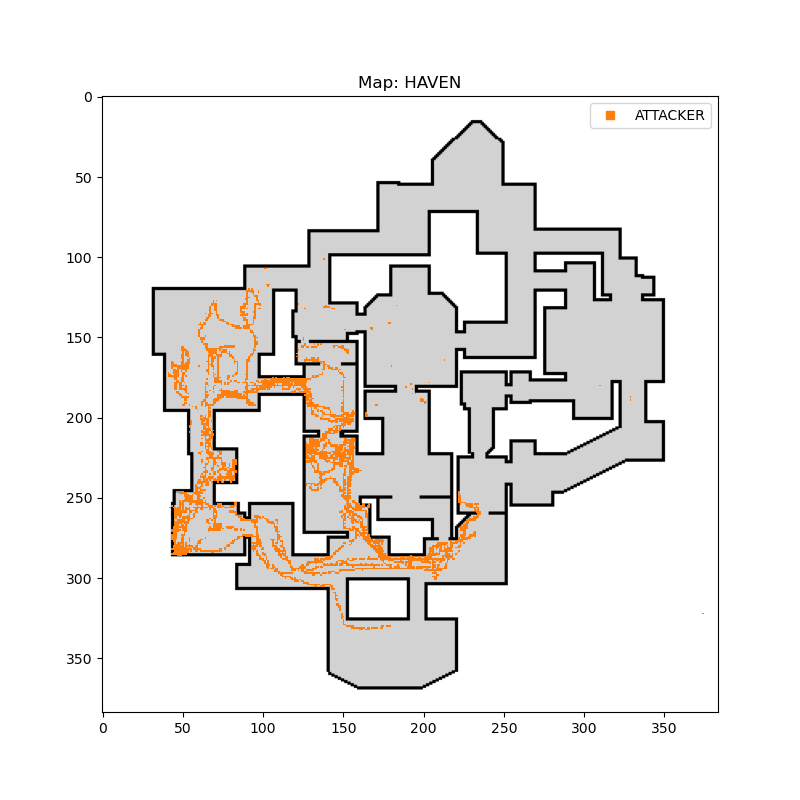
\includegraphics[width=0.95\linewidth]{images/a03-att-output}
	\caption[Output representation as map for attacker.]{Output representation as map, summarizing all positions 
		of attacker agents during one round on the map "Haven".}
	\label{fig:ea:outputAtt}
\end{figure}

\begin{figure}[H]
	\centering
	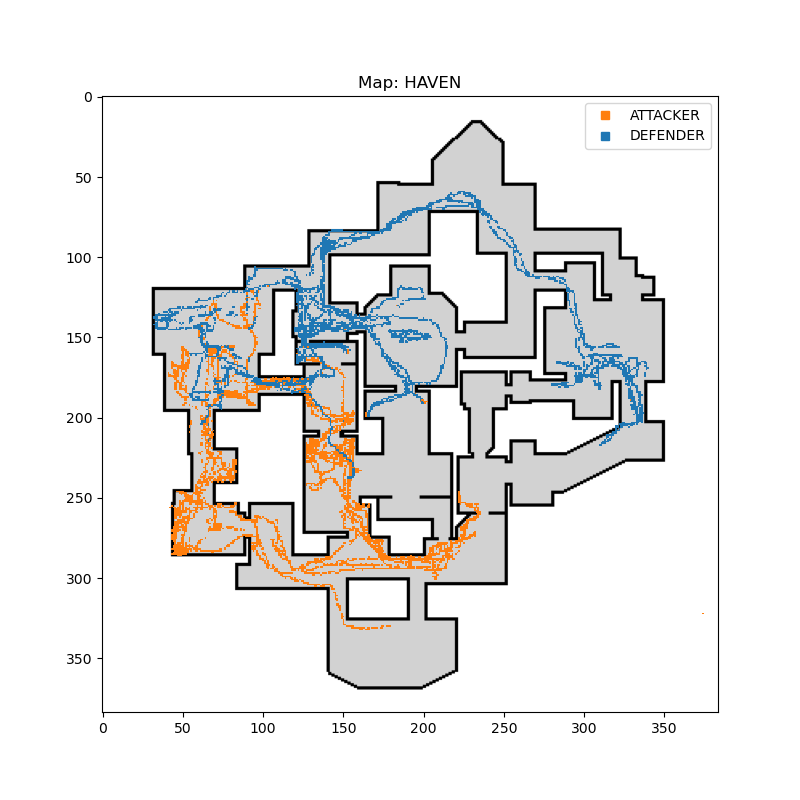
\includegraphics[width=0.95\linewidth]{images/a04-comb-output}
	\caption[Output representation as map.]{Output representation as map, summarizing all positions 
		of defender and attacker agents during one round on the map "Haven".}
	\label{fig:ea:outputComb}
\end{figure}

\backmatter
\printglossaries

\clearpage
\phantomsection
\addcontentsline{toc}{chapter}{\listfigurename}
\listoffigures

\clearpage
\phantomsection
\addcontentsline{toc}{chapter}{\listtablename}
\listoftables

%\renewcommand\lstlistlistingname{Codeverzeichnis}
%\clearpage
%\phantomsection
%\addcontentsline{toc}{chapter}{\lstlistlistingname}
%\lstlistoflistings
\printbibliography

\clearpage
\thispagestyle{empty}

Name: \fullname \hfill Matriculation number: \matnr \vspace{2cm}

\minisec{Statement}

I declare that I have independently written the thesis and have not used any sources or aids other 
than those specified.\vspace{2cm}

Ulm, \dotfill

\hspace{10cm} {\footnotesize \fullname}
\end{document}
